%!TEX root = ./soutenance.tex
\section[Décodeur logiciel à liste]{Décodage à liste sur processeurs généralistes}
\subsection*{}

\begin{frame}[c]{\'Evolutions des systèmes de télécommunications}
	\multiinclude[<+>][start=4,format=pdf,graphics={width=\textwidth}]{./fig/bs_evo}
	\begin{itemize}
		\item Architectures dédiées localisées pour le calcul bande de base
		\item Architectures dédiées à distance pour le calcul bande de base
		\item Cloud-RAN : décodeur logiciel
		\item Adaptativité de l'infrastructure
	\end{itemize}
\end{frame}

% \begin{frame}[c]{Décodeur logiciel}
% 	\begin{itemize}
% 		\vfill
% 		\item Architecture x86-64 majoritaire dans les serveurs
%     \vfill
%     \item Description logicielle du décodeur
%     \vfill
%     \item Exploiter les unités SIMD
% 		\vfill
% 		\item Meilleure efficacité énergétique : ARM
% 		\vfill
% 	\end{itemize}
% \end{frame}

\begin{frame}[c]{Généricité et Flexibilité}
  \vfill
	\begin{itemize}
		\item Généricité
		\begin{itemize}
			\item N, K
			\item Concaténation de CRC
			\item Position des bits gelés
			\item Poinçonnage
		\end{itemize}
    \vfill
		\item Flexibilité
		\begin{itemize}
			\item Variantes algorithmiques
			\item Taille de la liste
			\item Représentation en virgule fixe
			\item Ajustement de l'élagage
		\end{itemize}
	\end{itemize}
  \vfill
\end{frame}


\begin{frame}[c]{Généricité et Flexibilité}
    \centering

  \renewcommand*{\thefootnote}{\alph{footnote}}
  \begin{table}[t]
    {\small\resizebox{0.8\linewidth}{!}{
      \begin{tabular}{r|C{1cm}C{1cm}C{1cm}C{2cm}} 
       Décodeur     & \cite{shen_low-latency_2016} & \cite{sarkis_increasing_2014} & \cite{sarkis_fast_2016} & Ce travail  \\
      \cmidrule(lr){1-1}
      \cmidrule(lr){2-2}
      \cmidrule(lr){3-3}
      \cmidrule(lr){4-4}
      \cmidrule(lr){5-5}
       N               & \GREEN{\cmark}            & \GREEN{\cmark}                & \GREEN{\cmark}          & \GREEN{\cmark} \\
       K               & \GREEN{\cmark}            & \GREEN{\cmark}                & \GREEN{\cmark}          & \GREEN{\cmark} \\
       CRC             & \GREEN{\cmark}            & \GREEN{\cmark}                & \GREEN{\cmark}          & \GREEN{\cmark} \\
       Pos. bits gelés & \GREEN{\cmark}            & \GREEN{\cmark}                & \GREEN{\cmark}          & \GREEN{\cmark} \\
       Poinçonnage  & \xmark                       & \xmark                        & \xmark                  & \cmark \\
       \hline
       PASCL        & \xmark                       & \cmark                        & \cmark                  & \cmark \\
       FASCL        & \xmark                       & \xmark                        & \xmark                  & \cmark \\
       Virgule fixe & \xmark                       & \xmark                        & \xmark                  & \cmark \\
       \multirow{2}{*}{\'Elagage}    & \multirow{2}{*}{Fixe}                         &  \multirow{2}{*}{Fixe}                           &  \multirow{2}{*}{Fixe}                     & Ajustable \\
       & &  &  & Dynamique \\
       Code déroulé & NON                  & NON                   & OUI               & NON \\
       % Code déroulé & \GREEN{NON}                  & \GREEN{NON}                   & \RED{OUI}               & \GREEN{NON} \\

      \end{tabular}
    }}
  \end{table}


\end{frame}


\begin{frame}[c]{Généricité et Flexibilité}
    \centering

  \renewcommand*{\thefootnote}{\alph{footnote}}
      \only<1>{
      \begin{table}[t]
    {\small\resizebox{0.8\linewidth}{!}{
      \begin{tabular}{r|C{1cm}C{1cm}C{1cm}C{2cm}} 
       Décodeur     & \cite{shen_low-latency_2016} & \cite{sarkis_increasing_2014} & \cite{sarkis_fast_2016} & Ce travail  \\
      \cmidrule(lr){1-1}
      \cmidrule(lr){2-2}
      \cmidrule(lr){3-3}
      \cmidrule(lr){4-4}
      \cmidrule(lr){5-5}
       Poinçonnage  & {\xmark}                       & {\xmark}                        & {\xmark}                  & {\cmark} \\
       PASCL        & {\xmark}                       & {\cmark}                        & {\cmark}                  & {\cmark} \\
       FASCL        & {\xmark}                        & {\xmark}                        & {\xmark}                  & {\cmark} \\
       Virgule fixe & \xmark                       & \xmark                        & \xmark                  & \cmark \\
       \multirow{2}{*}{\'Elagage}    & \multirow{2}{*}{Fixe}                         &  \multirow{2}{*}{Fixe}                           &  \multirow{2}{*}{Fixe}                     & Ajustable \\
       & &  &  & Dynamique \\
       Latence ($\mu s$)\footnotemark[1]      &     1572  \footnotemark[2]                        & 3300  \footnotemark[3]                      & 433 \footnotemark[3]                 & 770 \footnotemark[3]\\
       Code déroulé & NON                  & NON                   & OUI               & NON \\
       % Code déroulé & \GREEN{NON}                  & \GREEN{NON}                   & \RED{OUI}               & \GREEN{NON} \\

      \end{tabular}
    }}
  \end{table}
  }    
  \only<2>{
      \begin{table}[t]
    {\small\resizebox{0.8\linewidth}{!}{
      \begin{tabular}{r|C{1cm}C{1cm}C{1cm}C{2cm}} 
       Décodeur     & \cite{shen_low-latency_2016} & \cite{sarkis_increasing_2014} & \cite{sarkis_fast_2016} & Ce travail  \\
      \cmidrule(lr){1-1}
      \cmidrule(lr){2-2}
      \cmidrule(lr){3-3}
      \cmidrule(lr){4-4}
      \cmidrule(lr){5-5}
       Poinçonnage  & \RED{\xmark}                       & \RED{\xmark}                        & \RED{\xmark}                  & \GREEN{\cmark} \\
       PASCL        & {\xmark}                       & {\cmark}                        & {\cmark}                  & {\cmark} \\
       FASCL        & {\xmark}                        & {\xmark}                        & {\xmark}                  & {\cmark} \\
       Virgule fixe & \xmark                       & \xmark                        & \xmark                  & \cmark \\
       \multirow{2}{*}{\'Elagage}    & \multirow{2}{*}{Fixe}                         &  \multirow{2}{*}{Fixe}                           &  \multirow{2}{*}{Fixe}                     & Ajustable \\
       & &  &  & Dynamique \\
       Latence ($\mu s$)\footnotemark[1]      &     1572  \footnotemark[2]                        & 3300  \footnotemark[3]                      & 433 \footnotemark[3]                 & 770 \footnotemark[3]\\
       Code déroulé & NON                  & NON                   & OUI               & NON \\
       % Code déroulé & \GREEN{NON}                  & \GREEN{NON}                   & \RED{OUI}               & \GREEN{NON} \\

      \end{tabular}
    }}
  \end{table}
  }    
  \only<3>{
      \begin{table}[t]
    {\small\resizebox{0.8\linewidth}{!}{
      \begin{tabular}{r|C{1cm}C{1cm}C{1cm}C{2cm}} 
       Décodeur     & \cite{shen_low-latency_2016} & \cite{sarkis_increasing_2014} & \cite{sarkis_fast_2016} & Ce travail  \\
      \cmidrule(lr){1-1}
      \cmidrule(lr){2-2}
      \cmidrule(lr){3-3}
      \cmidrule(lr){4-4}
      \cmidrule(lr){5-5}
       Poinçonnage  & \RED{\xmark}                       & \RED{\xmark}                        & \RED{\xmark}                  & \GREEN{\cmark} \\
       PASCL        & \RED{\xmark}                       & \GREEN{\cmark}                        & \GREEN{\cmark}                  & \GREEN{\cmark} \\
       FASCL        & \RED{\xmark}                        & \RED{\xmark}                        & \RED{\xmark}                  & \GREEN{\cmark} \\
       Virgule fixe & \xmark                       & \xmark                        & \xmark                  & \cmark \\
       \multirow{2}{*}{\'Elagage}    & \multirow{2}{*}{Fixe}                         &  \multirow{2}{*}{Fixe}                           &  \multirow{2}{*}{Fixe}                     & Ajustable \\
       & &  &  & Dynamique \\
       Latence ($\mu s$)\footnotemark[1]      &     1572  \footnotemark[2]                        & 3300  \footnotemark[3]                      & 433 \footnotemark[3]                 & 770 \footnotemark[3]\\
       Code déroulé & NON                  & NON                   & OUI               & NON \\
       % Code déroulé & \GREEN{NON}                  & \GREEN{NON}                   & \RED{OUI}               & \GREEN{NON} \\

      \end{tabular}
    }}
  \end{table}
  }
  \footnotetext[1]{CASCL, $K=1723$, $N=2048$} 
  \footnotetext[2]{Processeur Intel i7-4790K}
  \footnotetext[3]{Processeur Intel i7-2600} 
\end{frame}

\begin{frame}
\vfill
	\only<1>{
    \begin{table}[ht]
      \centering
      {\small\resizebox{0.8\linewidth}{!}{
      \begin{tabular}{r|c|c|c c c}
         \multirow{2}{*}{{Algorithme}} & \multirow{2}{*}{Version}  & \multirow{1}{*}{{${\mathcal{L}_{PC}}$}} & \multicolumn{3}{c}{Débit (Mb/s)} \\
        \cline{4-6}
        &   & ($\mu s$)            & {3.5 dB} & {4.0 dB} & {4.5 dB} \\
        \hline
        \textbf{PASCL} &~\cite{sarkis_increasing_2014}    & $\approx$ 3300                 & 0.9             & 4.90            & 54.0            \\
        \textbf{PASCL} &~\cite{sarkis_fast_2016}          & $\approx$ 433                  & 8.6             & 33.0            & 196.0           \\
        \textbf{PASCL} & Ce travail                       & 847                            & 5.5             & 31.1            & 168.4           \\
        \hline
        FASCL & Ce travail                       & 1602                           & 19.4            & 149.0           & 244.3           \\
      \end{tabular}
      }}
  	\end{table}
 	}

	\only<2>{
    \begin{table}[ht]
      \centering
      {\small\resizebox{0.8\linewidth}{!}{
      \begin{tabular}{r|c|c|c c c}
         \multirow{2}{*}{{Algorithme}} & \multirow{2}{*}{Version}  & \multirow{1}{*}{{${\mathcal{L}_{PC}}$}} & \multicolumn{3}{c}{Débit (Mb/s)} \\
        \cline{4-6}
        &   & ($\mu s$)            & {3.5 dB} & {4.0 dB} & {4.5 dB} \\
        \hline
        PASCL &~\cite{sarkis_increasing_2014}    & $\approx$ 3300                 & 0.9             & 4.90            & 54.0            \\
        PASCL &~\cite{sarkis_fast_2016}          & $\approx$ 433                  & 8.6             & 33.0            & 196.0           \\
        PASCL & Ce travail                       & 847                            & 5.5             & 31.1            & 168.4           \\
        \hline
        \textbf{FASCL} & Ce travail                       & 1602                           & 19.4            & 149.0           & 244.3           \\
      \end{tabular}
      }}
  	\end{table}
 	}
	\only<3>{
    \begin{table}[ht]
      \centering
      {\small\resizebox{0.8\linewidth}{!}{
      \begin{tabular}{r|c|c|c c c}
         \multirow{2}{*}{{Algorithme}} & \multirow{2}{*}{Version}  & \multirow{1}{*}{{${\mathcal{L}_{PC}}$}} & \multicolumn{3}{c}{Débit (Mb/s)} \\
        \cline{4-6}
        &   & ($\mu s$)            & {3.5 dB} & {4.0 dB} & {4.5 dB} \\
        \hline
        PASCL &~\cite{sarkis_increasing_2014}    & $\approx$ 3300                 & 0.9             & 4.90            & 54.0            \\
        PASCL &~\cite{sarkis_fast_2016}          & $\approx$ 433                  & 8.6             & 33.0            & 196.0           \\
        PASCL & Ce travail                       & \GREEN{847}                    & \ORANGE{5.5}             & \ORANGE{31.1}            & \ORANGE{168.4}           \\
        \hline
        FASCL & Ce travail                       & \RED{1602}                     & \GREEN{19.4}            & \GREEN{149.0}           & \GREEN{244.3}           \\
      \end{tabular}
      }}
  	\end{table}
 	}
	\only<4>{
    \begin{table}[ht]
      \centering
      {\small\resizebox{0.8\linewidth}{!}{
      \begin{tabular}{r|c|c|c c c}
         \multirow{2}{*}{{Algorithme}} & \multirow{2}{*}{Version}  & \multirow{1}{*}{{${\mathcal{L}_{PC}}$}} & \multicolumn{3}{c}{Débit (Mb/s)} \\
        \cline{4-6}
        &   & ($\mu s$)            & {3.5 dB} & {4.0 dB} & {4.5 dB} \\
        \hline
        PASCL &~\cite{sarkis_increasing_2014}    & $\approx$ 3300                 & \RED{0.9}       & \RED{4.90}      & \RED{54.0}      \\
        PASCL &~\cite{sarkis_fast_2016}          & $\approx$ 433                  & \ORANGE{8.6}    & \ORANGE{33.0 }  & \ORANGE{196.0}  \\
        PASCL & Ce travail                       & 847                            & \ORANGE{5.5}    & \ORANGE{31.1}   & \ORANGE{168.4}  \\
        \hline
        FASCL & Ce travail                       & 1602                           & \GREEN{19.4}    & \GREEN{149.0}   & \GREEN{244.3}   \\
      \end{tabular}
      }}
  	\end{table}
 	}
 	\vfill

  \begin{itemize}
  	\item<+-> Algorithme partiellement adaptatif (PASCL)
  	\item<+-> Algorithme complètement adaptatif (FASCL)
  	\item<+-> Compromis latence vs débit
  	\item<+-> Algorithme FASCL propose les plus hauts débits
  \end{itemize}
  \vfill
\end{frame}


\begin{frame}[c]{Généricité et Flexibilité}
  \renewcommand*{\thefootnote}{\alph{footnote}}

    \centering
    \only<1>{
      \begin{table}[t]
    {\small\resizebox{0.8\linewidth}{!}{
     	\begin{tabular}{r|C{1cm}C{1cm}C{1cm}C{2cm}} 
     	 Décodeur     & \cite{shen_low-latency_2016} & \cite{sarkis_increasing_2014} & \cite{sarkis_fast_2016} & Ce travail  \\
     	\cmidrule(lr){1-1}
     	\cmidrule(lr){2-2}
     	\cmidrule(lr){3-3}
     	\cmidrule(lr){4-4}
     	\cmidrule(lr){5-5}
     	 Poinçonnage  & \RED{\xmark}                       & \RED{\xmark}                        & \RED{\xmark}                  & \GREEN{\cmark} \\
     	 PASCL        & \RED{\xmark}                       & \GREEN{\cmark}                        & \GREEN{\cmark}                  & \GREEN{\cmark} \\
     	 FASCL        & \RED{\xmark}                        & \RED{\xmark}                        & \RED{\xmark}                  & \GREEN{\cmark} \\
     	 Virgule fixe & \xmark                       & \xmark                        & \xmark                  & \cmark \\
     	 \multirow{2}{*}{\'Elagage}    & \multirow{2}{*}{Fixe}                         &  \multirow{2}{*}{Fixe}                           &  \multirow{2}{*}{Fixe}                     & Ajustable \\
     	 & &  &  & Dynamique \\
     	 Latence ($\mu s$)\footnotemark[1]      &     1572  \footnotemark[2]                        & 3300  \footnotemark[3]                      & 433 \footnotemark[3]                 & 770 \footnotemark[3]\\
     	 Code déroulé & NON                  & NON                   & OUI               & NON \\
     	 % Code déroulé & \GREEN{NON}                  & \GREEN{NON}                   & \RED{OUI}               & \GREEN{NON} \\

    	\end{tabular}
    }}
  \end{table}
  }
    \only<2>{
  \begin{table}[t]
    {\small\resizebox{0.8\linewidth}{!}{
     	\begin{tabular}{r|C{1cm}C{1cm}C{1cm}C{2cm}} 
     	 Décodeur     & \cite{shen_low-latency_2016} & \cite{sarkis_increasing_2014} & \cite{sarkis_fast_2016} & Ce travail  \\
     	\cmidrule(lr){1-1}
     	\cmidrule(lr){2-2}
     	\cmidrule(lr){3-3}
     	\cmidrule(lr){4-4}
     	\cmidrule(lr){5-5}
     	 Poinçonnage  & \RED{\xmark}                       & \RED{\xmark}                        & \RED{\xmark}                  & \GREEN{\cmark} \\
     	 PASCL        & \RED{\xmark}                       & \GREEN{\cmark}                        & \GREEN{\cmark}                  & \GREEN{\cmark} \\
     	 FASCL        & \RED{\xmark}                        & \RED{\xmark}                        & \RED{\xmark}                  & \GREEN{\cmark} \\
     	 Virgule fixe & \RED{\xmark}                       & \RED{\xmark}                        & \RED{\xmark}                  & \GREEN{\cmark} \\
     	 \multirow{2}{*}{\'Elagage}    & \multirow{2}{*}{Fixe}                         &  \multirow{2}{*}{Fixe}                           &  \multirow{2}{*}{Fixe}                     & Ajustable \\
     	 & &  &  & Dynamique \\
     	 Latence ($\mu s$)\footnotemark[1]      &     1572  \footnotemark[2]                        & 3300  \footnotemark[3]                      & 433 \footnotemark[3]                 & 770 \footnotemark[3]\\
     	 Code déroulé & NON                  & NON                   & OUI               & NON \\
     	 % Code déroulé & \GREEN{NON}                  & \GREEN{NON}                   & \RED{OUI}               & \GREEN{NON} \\

    	\end{tabular}
    }}
  \end{table}
  }
  \footnotetext[1]{CASCL, $K=1723$, $N=2048$} 
  \footnotetext[2]{Processeur Intel i7-4790K}
  \footnotetext[3]{Processeur Intel i7-2600} 
\end{frame}
  

\begin{frame}[c]{Représentation en virgule fixe}

    \only<+>
    {
  \begin{table}[hb]
    \renewcommand{\arraystretch}{1.2}
    \centering
    {\small\resizebox{0.6\linewidth}{!}{
    \begin{tabular}{r | c  || c | c | c }
      \multirow{2}{*}{\textbf{Décodeur}} & \multirow{2}{*}{\textbf{Quantif.}}  & \multicolumn{3}{c}{Débit (Mb/s)}  \\
      \cline{3-5}
      & &  $\mathbold{\frac{E_b}{n_0} = 3.5} \text{dB}$ & $\mathbold{\frac{E_b}{n_0} = 4.0} \text{dB}$ & $\mathbold{\frac{E_b}{n_0} = 4.5} \text{dB}$ \\
      % \hline
      \hline
      \multirow{3}{*}{PASCL} & 32-bit   &   7.6 &   42.1 &  237.6 \\
      %\cline{3-9}
                               & 16-bit   &   8.0 &   43.8 &  267.5 \\
      %\cline{3-9}
                               &  8-bit &   7.6 &   42.6 &  268.3 \\
      \hline
      \multirow{3}{*}{FASCL}  & 32-bit   &  26.1 &  207.8 &  345.5 \\
      %\cline{3-9}
                               & 16-bit   &  25.6 &  225.7 &  408.7 \\
      %\cline{3-9}
                               &  8-bit   &  24.4 &  227.3 &  425.9 \\
    \end{tabular}
    }}
   \end{table}

   }
    \only<+>
    {
      \begin{table}[hb]
    \renewcommand{\arraystretch}{1.2}
    \centering
    {\small\resizebox{0.6\linewidth}{!}{
    \begin{tabular}{r | c  || c | c | c }
      \multirow{2}{*}{\textbf{Décodeur}} & \multirow{2}{*}{\textbf{Quantif.}}  & \multicolumn{3}{c}{Débit (Mb/s)}  \\
      \cline{3-5}
      & &  $\mathbold{\frac{E_b}{n_0} = 3.5} \text{dB}$ & $\mathbold{\frac{E_b}{n_0} = 4.0} \text{dB}$ & $\mathbold{\frac{E_b}{n_0} = 4.5} \text{dB}$ \\
      % \hline
      \hline
      \multirow{3}{*}{PASCL} & 32-bit   &   7.6 &   42.1 &  237.6 \\
      %\cline{3-9}
                               & 16-bit   &   8.0 &   43.8 &  267.5 \\
      %\cline{3-9}
                               &  8-bit &   7.6 &   42.6 &  268.3 \\
      \hline
      \multirow{3}{*}{FASCL}  & \RED{32-bit}   &  26.1 &  207.8 &  \RED{345.5} \\
      %\cline{3-9}
                               & \ORANGE{16-bit}   &  25.6 &  225.7 &  \ORANGE{408.7} \\
      %\cline{3-9}
                               &  \GREEN{8-bit}   &  24.4 &  227.3 &  \GREEN{425.9} \\
    \end{tabular}
    }}
   \end{table}
   }
    \begin{itemize}
    	\item Prototypage
    	\item Augmentation du parallélisme
    	\item Augmentation du débit
    \end{itemize}
\end{frame}


\begin{frame}[c]{Généricité et Flexibilité}
  \renewcommand*{\thefootnote}{\alph{footnote}}

    \centering
    \only<1>{
      \begin{table}[t]
    {\small\resizebox{0.8\linewidth}{!}{
     	\begin{tabular}{r|C{1cm}C{1cm}C{1cm}C{2cm}} 
     	 Décodeur     & \cite{shen_low-latency_2016} & \cite{sarkis_increasing_2014} & \cite{sarkis_fast_2016} & Ce travail  \\
     	\cmidrule(lr){1-1}
     	\cmidrule(lr){2-2}
     	\cmidrule(lr){3-3}
     	\cmidrule(lr){4-4}
     	\cmidrule(lr){5-5}
     	 Poinçonnage  & \RED{\xmark}                       & \RED{\xmark}                        & \RED{\xmark}                  & \GREEN{\cmark} \\
     	 PASCL        & \RED{\xmark}                       & \GREEN{\cmark}                        & \GREEN{\cmark}                  & \GREEN{\cmark} \\
     	 FASCL        & \RED{\xmark}                        & \RED{\xmark}                        & \RED{\xmark}                  & \GREEN{\cmark} \\
     	 Virgule fixe & \RED{\xmark}                       & \RED{\xmark}                        & \RED{\xmark}                  & \GREEN{\cmark} \\
     	 \multirow{2}{*}{\'Elagage}    & \multirow{2}{*}{Fixe}                         &  \multirow{2}{*}{Fixe}                           &  \multirow{2}{*}{Fixe}                     & Ajustable \\
     	 & &  &  & Dynamique \\
     	 Latence ($\mu s$)\footnotemark[1]      &     1572  \footnotemark[2]                        & 3300  \footnotemark[3]                      & 433 \footnotemark[3]                 & 770 \footnotemark[3]\\
     	 Code déroulé & NON                  & NON                   & OUI               & NON \\
     	 % Code déroulé & \GREEN{NON}                  & \GREEN{NON}                   & \RED{OUI}               & \GREEN{NON} \\

    	\end{tabular}
    }}
  \end{table}
    }
    \only<2>
    {
  \begin{table}[t]
    {\small\resizebox{0.8\linewidth}{!}{
     	\begin{tabular}{r|C{1cm}C{1cm}C{1cm}C{2cm}} 
     	 Décodeur     & \cite{shen_low-latency_2016} & \cite{sarkis_increasing_2014} & \cite{sarkis_fast_2016} & Ce travail  \\
     	\cmidrule(lr){1-1}
     	\cmidrule(lr){2-2}
     	\cmidrule(lr){3-3}
     	\cmidrule(lr){4-4}
     	\cmidrule(lr){5-5}
     	 Poinçonnage  & \RED{\xmark}                       & \RED{\xmark}                        & \RED{\xmark}                  & \GREEN{\cmark} \\
     	 PASCL        & \RED{\xmark}                       & \GREEN{\cmark}                        & \GREEN{\cmark}                  & \GREEN{\cmark} \\
     	 FASCL        & \RED{\xmark}                        & \RED{\xmark}                        & \RED{\xmark}                  & \GREEN{\cmark} \\
     	 Virgule fixe & \RED{\xmark}                       & \RED{\xmark}                        & \RED{\xmark}                  & \GREEN{\cmark} \\
     	 \multirow{2}{*}{\'Elagage}    & \multirow{2}{*}{ \RED{Fixe}}                         &  \multirow{2}{*}{ \RED{Fixe}}                           &  \multirow{2}{*}{ \RED{Fixe}}                     & \GREEN{Ajustable} \\
     	 & &  &  & \GREEN{Dynamique} \\
     	 Latence ($\mu s$)\footnotemark[1]      &     1572  \footnotemark[2]                        & 3300  \footnotemark[3]                      & 433 \footnotemark[3]                 & 770 \footnotemark[3]\\
     	 Code déroulé & NON                  & NON                   & OUI               & NON \\
     	 % Code déroulé & \GREEN{NON}                  & \GREEN{NON}                   & \RED{OUI}               & \GREEN{NON} \\

    	\end{tabular}
    }}
  \end{table}
  }
  \footnotetext[1]{CASCL, $K=1723$, $N=2048$} 
  \footnotetext[2]{Processeur Intel i7-4790K}
  \footnotetext[3]{Processeur Intel i7-2600} 
\end{frame}


  \begin{frame}[c]{Impact de l'élagage des nœuds SPC}
	\centering
  \multiinclude[<+>][start=1,format=pdf,graphics={width=\textwidth}]{./fig/thr_spc/tikz/source}
\end{frame}

\begin{frame}[c]{Généricité et Flexibilité}
  \renewcommand*{\thefootnote}{\alph{footnote}}

    \centering
  \only<1>{
  \begin{table}[t]
    {\small\resizebox{0.8\linewidth}{!}{
     	\begin{tabular}{r|C{1cm}C{1cm}C{1cm}C{2cm}} 
     	 Décodeur     & \cite{shen_low-latency_2016} & \cite{sarkis_increasing_2014} & \cite{sarkis_fast_2016} & Ce travail  \\
     	\cmidrule(lr){1-1}
     	\cmidrule(lr){2-2}
     	\cmidrule(lr){3-3}
     	\cmidrule(lr){4-4}
     	\cmidrule(lr){5-5}
     	 Poinçonnage  & \RED{\xmark}                       & \RED{\xmark}                        & \RED{\xmark}                  & \GREEN{\cmark} \\
     	 PASCL        & \RED{\xmark}                       & \GREEN{\cmark}                        & \GREEN{\cmark}                  & \GREEN{\cmark} \\
     	 FASCL        & \RED{\xmark}                        & \RED{\xmark}                        & \RED{\xmark}                  & \GREEN{\cmark} \\
     	 Virgule fixe & \RED{\xmark}                       & \RED{\xmark}                        & \RED{\xmark}                  & \GREEN{\cmark} \\
     	 \multirow{2}{*}{\'Elagage}    & \multirow{2}{*}{ \RED{Fixe}}                         &  \multirow{2}{*}{ \RED{Fixe}}                           &  \multirow{2}{*}{ \RED{Fixe}}                     & \GREEN{Ajustable} \\
     	 & &  &  & \GREEN{Dynamique} \\
     	 Latence ($\mu s$)\footnotemark[1]      &     1572  \footnotemark[2]                        & 3300  \footnotemark[3]                      & 433 \footnotemark[3]                 & 770 \footnotemark[3]\\
     	 Code déroulé & NON                  & NON                   & OUI               & NON \\
     	 % Code déroulé & \GREEN{NON}                  & \GREEN{NON}                   & \RED{OUI}               & \GREEN{NON} \\

    	\end{tabular}
    }}
  \end{table}
  }
  \only<2>
  {
  \begin{table}[t]
    {\small\resizebox{0.8\linewidth}{!}{
     	\begin{tabular}{r|C{1cm}C{1cm}C{1cm}C{2cm}} 
     	 Décodeur     & \cite{shen_low-latency_2016} & \cite{sarkis_increasing_2014} & \cite{sarkis_fast_2016} & Ce travail  \\
     	\cmidrule(lr){1-1}
     	\cmidrule(lr){2-2}
     	\cmidrule(lr){3-3}
     	\cmidrule(lr){4-4}
     	\cmidrule(lr){5-5}
     	 Poinçonnage  & \RED{\xmark}                       & \RED{\xmark}                        & \RED{\xmark}                  & \GREEN{\cmark} \\
     	 PASCL        & \RED{\xmark}                       & \GREEN{\cmark}                        & \GREEN{\cmark}                  & \GREEN{\cmark} \\
     	 FASCL        & \RED{\xmark}                        & \RED{\xmark}                        & \RED{\xmark}                  & \GREEN{\cmark} \\
     	 Virgule fixe & \RED{\xmark}                       & \RED{\xmark}                        & \RED{\xmark}                  & \GREEN{\cmark} \\
     	 \multirow{2}{*}{\'Elagage}    & \multirow{2}{*}{ \RED{Fixe}}                         &  \multirow{2}{*}{ \RED{Fixe}}                           &  \multirow{2}{*}{ \RED{Fixe}}                     & \GREEN{Ajustable} \\
     	 & &  &  & \GREEN{Dynamique} \\
     	 Latence ($\mu s$)\footnotemark[1]      &     \RED{1572}  \footnotemark[2]                        & \RED{3300}  \footnotemark[3]                      & \GREEN{433} \footnotemark[3]                 & \ORANGE{770} \footnotemark[3]\\
     	 Code déroulé & NON                  & NON                   & OUI               & NON \\
     	 % Code déroulé & \GREEN{NON}                  & \GREEN{NON}                   & \RED{OUI}               & \GREEN{NON} \\

    	\end{tabular}
    }}
  \end{table}
  }
  \only<3>
  {
  \begin{table}[t]
    {\small\resizebox{0.8\linewidth}{!}{
     	\begin{tabular}{r|C{1cm}C{1cm}C{1cm}C{2cm}} 
     	 Décodeur     & \cite{shen_low-latency_2016} & \cite{sarkis_increasing_2014} & \cite{sarkis_fast_2016} & Ce travail  \\
     	\cmidrule(lr){1-1}
     	\cmidrule(lr){2-2}
     	\cmidrule(lr){3-3}
     	\cmidrule(lr){4-4}
     	\cmidrule(lr){5-5}
     	 Poinçonnage  & \RED{\xmark}                       & \RED{\xmark}                        & \RED{\xmark}                  & \GREEN{\cmark} \\
     	 PASCL        & \RED{\xmark}                       & \GREEN{\cmark}                        & \GREEN{\cmark}                  & \GREEN{\cmark} \\
     	 FASCL        & \RED{\xmark}                        & \RED{\xmark}                        & \RED{\xmark}                  & \GREEN{\cmark} \\
     	 Virgule fixe & \RED{\xmark}                       & \RED{\xmark}                        & \RED{\xmark}                  & \GREEN{\cmark} \\
     	 \multirow{2}{*}{\'Elagage}    & \multirow{2}{*}{ \RED{Fixe}}                         &  \multirow{2}{*}{ \RED{Fixe}}                           &  \multirow{2}{*}{ \RED{Fixe}}                     & \GREEN{Ajustable} \\
     	 & &  &  & \GREEN{Dynamique} \\
     	 Latence ($\mu s$)\footnotemark[1]      &     \RED{1572}  \footnotemark[2]                        & \RED{3300}  \footnotemark[3]                      & \GREEN{433} \footnotemark[3]                 & \ORANGE{770} \footnotemark[3]\\
     	 Code déroulé & \GREEN{NON}                  & \GREEN{NON}                   & \RED{OUI}               & \GREEN{NON} \\
     	 % Code déroulé & \GREEN{NON}                  & \GREEN{NON}                   & \RED{OUI}               & \GREEN{NON} \\

    	\end{tabular}
    }}
  \end{table}
  }
  \footnotetext[1]{CASCL, $K=1723$, $N=2048$} 
  \footnotetext[2]{Processeur Intel i7-4790K}
  \footnotetext[3]{Processeur Intel i7-2600} 
\end{frame}


\begin{frame}[c]{Déroulage}
	\multiinclude[<+>][start=1,format=pdf,graphics={width=\textwidth}]{./fig/unrolling}
\end{frame}

\begin{frame}[c]{Déroulage}
\begin{center}
			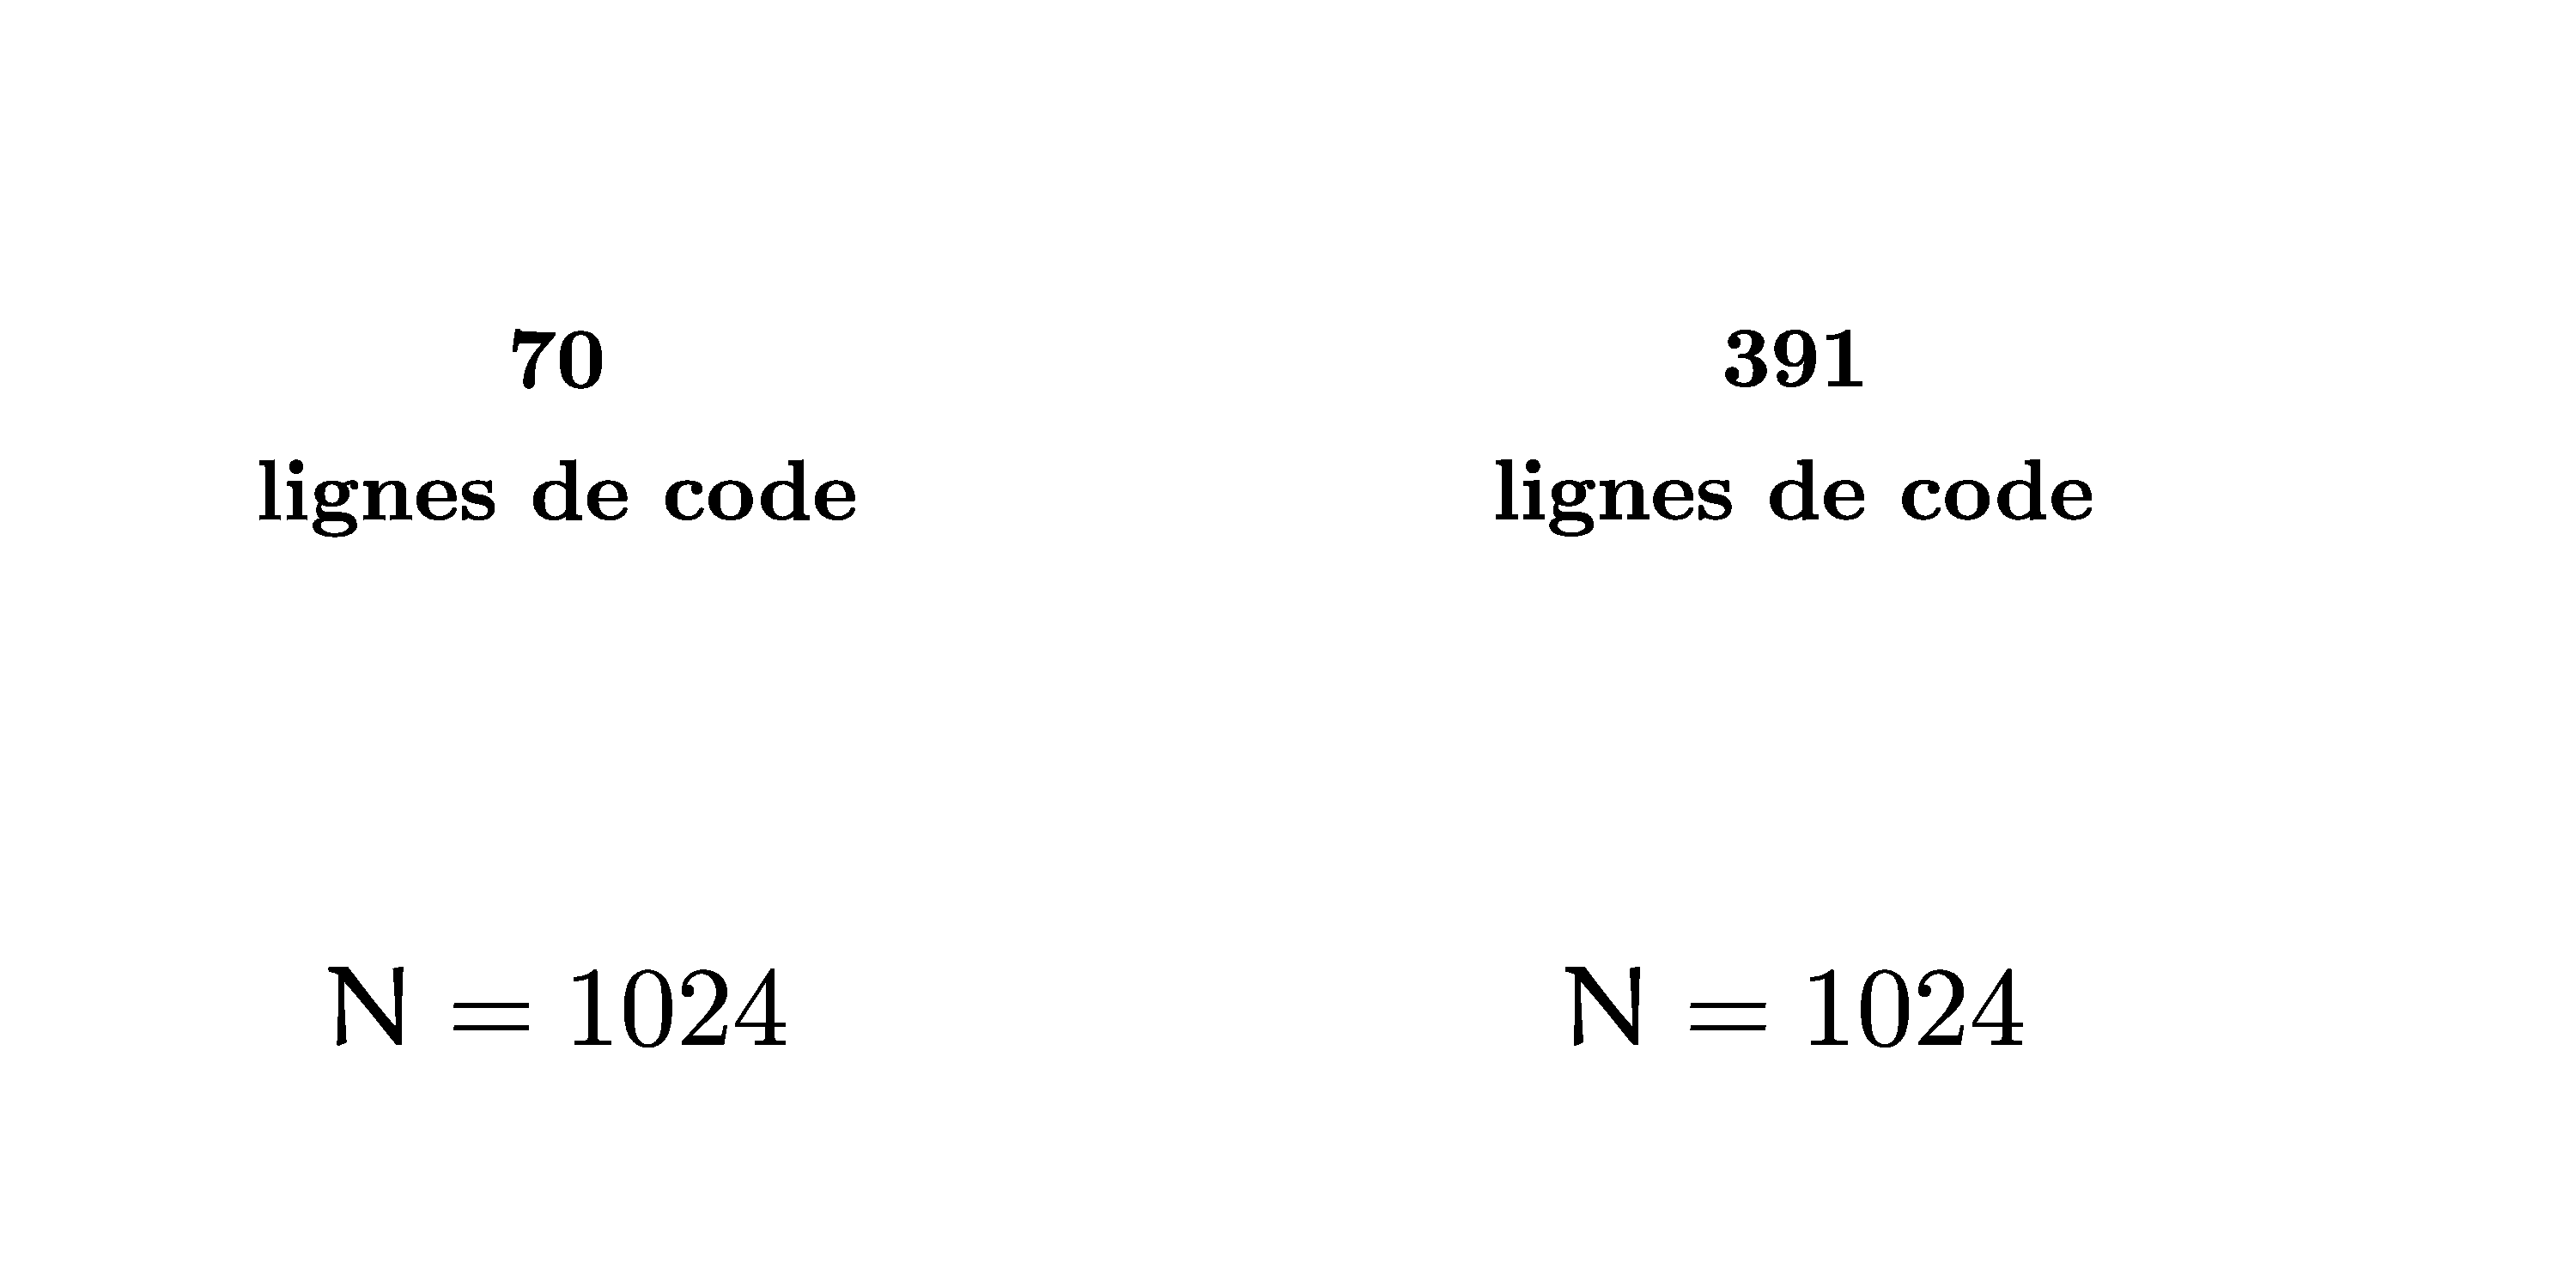
\includegraphics[width=.5\textwidth]{./fig/unrolling-4}
\end{center}

  \begin{itemize}
    \vfill
    \item \GREEN{+ \'Evite indirections}
    \vfill
    \item \GREEN{+ Diminue le temps de décodage}
    \vfill
    \item \RED{- Une version du code par jeu de paramètres}
    \vfill
    \item \RED{- Augmentation drastique de la taille du code}
    \vfill
    \item \RED{- Difficilement compatible dans le contexte 5G}
    \vfill
  \end{itemize}
\end{frame}


\begin{frame}[c]{Généricité et Flexibilité}
  \renewcommand*{\thefootnote}{\alph{footnote}}

    \centering
  \begin{table}[t]
    {\small\resizebox{0.8\linewidth}{!}{
     	\begin{tabular}{r|C{1cm}C{1cm}C{1cm}C{2cm}} 
     	 Décodeur     & \cite{shen_low-latency_2016} & \cite{sarkis_increasing_2014} & \cite{sarkis_fast_2016} & Ce travail  \\
     	\cmidrule(lr){1-1}
     	\cmidrule(lr){2-2}
     	\cmidrule(lr){3-3}
     	\cmidrule(lr){4-4}
     	\cmidrule(lr){5-5}
     	 Poinçonnage  & \RED{\xmark}                       & \RED{\xmark}                        & \RED{\xmark}                  & \GREEN{\cmark} \\
     	 PASCL        & \RED{\xmark}                       & \GREEN{\cmark}                        & \GREEN{\cmark}                  & \GREEN{\cmark} \\
     	 FASCL        & \RED{\xmark}                        & \RED{\xmark}                        & \RED{\xmark}                  & \GREEN{\cmark} \\
     	 Virgule fixe & \RED{\xmark}                       & \RED{\xmark}                        & \RED{\xmark}                  & \GREEN{\cmark} \\
     	 \multirow{2}{*}{\'Elagage}    & \multirow{2}{*}{ \RED{Fixe}}                         &  \multirow{2}{*}{ \RED{Fixe}}                           &  \multirow{2}{*}{ \RED{Fixe}}                     & \GREEN{Ajustable} \\
     	 & &  &  & \GREEN{Dynamique} \\
     	 Latence ($\mu s$)\footnotemark[1]      &     \RED{1572}  \footnotemark[2]                        & \RED{3300}  \footnotemark[3]                      & \GREEN{433} \footnotemark[3]                 & \ORANGE{770} \footnotemark[3]\\
     	 Code déroulé & \GREEN{NON}                  & \GREEN{NON}                   & \RED{OUI}               & \GREEN{NON} \\
     	 % Code déroulé & \GREEN{NON}                  & \GREEN{NON}                   & \RED{OUI}               & \GREEN{NON} \\

    	\end{tabular}
    }}
  \end{table}
  
  \footnotetext[1]{CASCL, $K=1723$, $N=2048$} 
  \footnotetext[2]{Processeur Intel i7-4790K}
  \footnotetext[3]{Processeur Intel i7-2600} 
\end{frame}

\begin{frame}[c]{Accélération du décodage logiciel}
\only<+>{
	\begin{itemize}
		\vfill
		\item Extraction du CRC
		\vfill
		\item Nouvelle méthode de tri
		\vfill
		\item Gestion du stockage des sommes partielles
		\vfill
	\end{itemize}
  }
  \only<+>
  {
	\begin{itemize}
		\vfill
		\item \textbf{Extraction du CRC}
		\vfill
		\item Nouvelle méthode de tri
		\vfill
		\item Gestion du stockage des sommes partielles
		\vfill
	\end{itemize}
  }
	% \footnotetext[1]{https://aff3ct.github.io}
\end{frame}


\begin{frame}
\vfill
\centering
  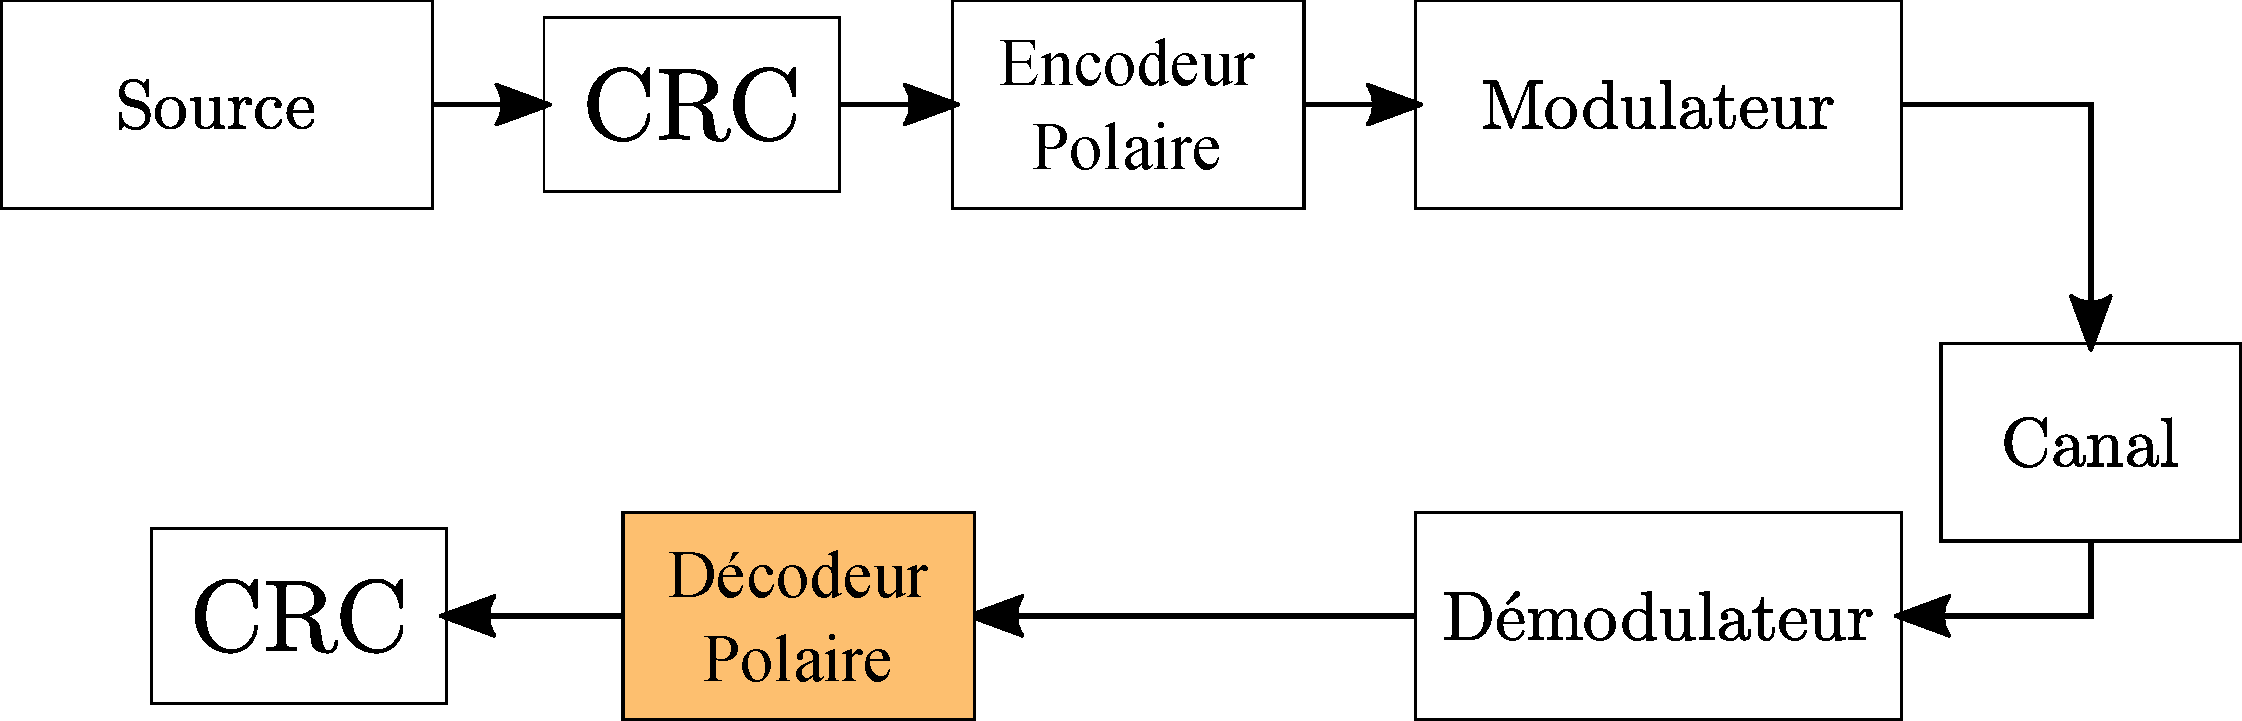
\includegraphics[width=0.7\textwidth]{./fig/extract-1}
  \vfill
\end{frame}

\begin{frame}[c]{Extraction du CRC}
	\centering
	\multiinclude[<+>][start=2,format=pdf,graphics={width=.7\textwidth}]{./fig/extract}
\end{frame}

\begin{frame}[c]{Résumé}
	\begin{itemize}
		\vfill
		\item Les décodeurs logiciels pour les systèmes de communication
		\vfill
		\item Généricité et Flexibilité
		\vfill
		\item Comparaison avec l'état de l'art
		\vfill
		\item Améliorations du débit et de la latence
		\vfill
    \item Mise à disposition du code source \footnote{https://aff3ct.github.io}
    \vfill
		\item Consommation \'Energétique ?
		\vfill
	\end{itemize}
\end{frame}

\begin{frame}[c]{Consommation énergétique}

	\begin{minipage}[c][0cm][t]{\textwidth}
	\centering
	\vfill
	\only<1>{Implémentations logicielles sur des processeurs généralistes}
	\vfill
	\only<2>{Implémentations matérielles dédiées}
	\vfill
	\only<3>{Tailles de codes et rendements variés}
	\vfill
	\only<5>{Débits compétitifs des décodeurs logiciels}
	\vfill
	\only<6>{Principal défaut des décodeurs logiciels : la consommation énergétique}
	\vfill
	\only<7>{\GREEN{Comment conserver la flexibilité des décodeurs logiciels en se rapprochant des performances des architectures dédiées ?}}
	\vfill
	\end{minipage}		

	\vspace{1cm}
\centering
	\only<+>{
  \begin{table}[t]
  \begin{tabular}{C{0.9cm}|C{1.9cm}|C{1cm}|C{0.7cm}|C{1.7cm}|C{1.5cm}}
  Ref.           & \textbf{Circuit  } &  N                     & R            & Débit (Mb/s) & $E_b$ (nJ/bit)  \\\hline
  \cite{Giard15} & \textbf{i7-4770S  } &  32768                 & 0.84        & 886        & 73              \\
  \cite{6960078} & \textbf{i7-4960HQ } &  32768                 & 0.83        & 1400       & 34              \\
  \cite{7760327} & \textbf{Cortex A57} &  32768                 & 0.83        & 73         & 27              \\\hline
  \cite{6804939} & Stratix IV &  32768                 & 0.9                  & 1200       & -                        \\
  \cite{7105452} & Stratix IV &  1024\footnotemark[1]  & 0.5\footnotemark[1]  & 237000     & -                        \\
  \cite{8017407} & ASIC 28nm  &  1024                  & 0.5                  & 94         & 0.095                    \\
  \cite{8017407} & ASIC 28nm  &  1024\footnotemark[1]  & 0.5\footnotemark[1]  & 436        & 0.006                    \\
  \end{tabular}
  \end{table}
  \footnotetext[1]{\tiny Fixed N \& R}
  }
  \only<+>{
  \begin{table}[t]
  \begin{tabular}{C{0.9cm}|C{1.9cm}|C{1cm}|C{0.7cm}|C{1.7cm}|C{1.5cm}}
	Ref.           & \textbf{Circuit} &  N                     & R                       & Débit (Mb/s) & $E_b$ (nJ/bit)  \\\hline
	\cite{Giard15} & i7-4770S   &  32768                 & 0.84                          & 886        & 73                       \\
	\cite{6960078} & i7-4960HQ  &  32768                 & 0.83                          & 1400       & 34                       \\
	\cite{7760327} & Cortex A57 &  32768                 & 0.83                          & 73         & 27                       \\\hline
	\cite{6804939} & \textbf{Stratix IV} &  32768                 & 0.9                  & 1200       & -               \\
	\cite{7105452} & \textbf{Stratix IV} &  1024\footnotemark[1]  & 0.5\footnotemark[1]  & 237000     & -               \\
	\cite{8017407} & \textbf{ASIC 28nm } &  1024                  & 0.5                  & 94         & 0.095           \\
	\cite{8017407} & \textbf{ASIC 28nm } &  1024\footnotemark[1]  & 0.5\footnotemark[1]  & 436        & 0.006           \\
	\end{tabular}
  \end{table}

	\footnotetext[1]{\tiny Fixed N \& R}
	}
	\only<+>{
  \begin{table}[t]
  \begin{tabular}{C{0.9cm}|C{1.9cm}|C{1cm}|C{0.7cm}|C{1.7cm}|C{1.5cm}}
	Ref.           & Circuit   &  \textbf{N                  }   & \textbf{R                  }   & Débit (Mb/s) & $E_b$ (nJ/bit)  \\\hline
	\cite{Giard15} & i7-4770S   &  \textbf{32768              }   & \textbf{0.84               }  & 886        & 73              \\
	\cite{6960078} & i7-4960HQ  &  \textbf{32768              }   & \textbf{0.83               }  & 1400       & 34              \\
	\cite{7760327} & Cortex A57 &  \textbf{32768              }   & \textbf{0.83               }  & 73         & 27              \\\hline
	\cite{6804939} & Stratix IV &  \textbf{32768              }   & \textbf{0.9                }  & 1200       & -               \\
	\cite{7105452} & Stratix IV &  \textbf{1024\footnotemark[1]}  & \textbf{0.5\footnotemark[1]}  & 237000     & -               \\
	\cite{8017407} & ASIC 28nm  &  \textbf{1024               }   & \textbf{0.5                }  & 94         & 0.095           \\
	\cite{8017407} & ASIC 28nm  &  \textbf{1024\footnotemark[1]}  & \textbf{0.5\footnotemark[1]}  & 436        & 0.006           \\
	\end{tabular}
  \end{table}

	\footnotetext[1]{\tiny Fixed N \& R}
	}

	\only<+>{
  \begin{table}[t]
  \begin{tabular}{C{0.9cm}|C{1.9cm}|C{1cm}|C{0.7cm}|C{1.7cm}|C{1.5cm}}
	Ref.           & Circuit   &  N                     & R                     & \textbf{Débit (Mb/s)} & $E_b$ (nJ/bit)    \\\hline
	\cite{Giard15} & i7-4770S   &  32768                 & 0.84                 & \GREEN{886}        & 73                 \\
	\cite{6960078} & i7-4960HQ  &  32768                 & 0.83                 & \GREEN{1400}       & 34                 \\
	\cite{7760327} & Cortex A57 &  32768                 & 0.83                 & \ORANGE{73}        & 27                 \\\hline
	\cite{6804939} & Stratix IV &  32768                 & 0.9                  & \GREEN{1200}       & -                  \\
	\cite{7105452} & Stratix IV &  1024\footnotemark[1]  & 0.5\footnotemark[1]  & \BLUE{237000}      & -                  \\
	\cite{8017407} & ASIC 28nm  &  1024                  & 0.5                  & \ORANGE{94}        & 0.095              \\
	\cite{8017407} & ASIC 28nm  &  1024\footnotemark[1]  & 0.5\footnotemark[1]  & \GREEN{436}        & 0.006              \\
	\end{tabular}
  \end{table}

	\footnotetext[1]{\tiny Fixed N \& R}
	}
	\only<+>{
  \begin{table}[t]
  \begin{tabular}{C{0.9cm}|C{1.9cm}|C{1cm}|C{0.7cm}|C{1.7cm}|C{1.5cm}}
	Ref.           & Circuit   &  N                     & R                     & Débit (Mb/s) & $\mathbf{E_b}$ \textbf{(nJ/bit)}  \\\hline
	\cite{Giard15} & i7-4770S   &  32768                 & 0.84                 & 886        & \ORANGE{73}                       \\
	\cite{6960078} & i7-4960HQ  &  32768                 & 0.83                 & 1400       & \ORANGE{34}                       \\
	\cite{7760327} & Cortex A57 &  32768                 & 0.83                 & 73         & \ORANGE{27}                       \\\hline
	\cite{6804939} & Stratix IV &  32768                 & 0.9                  & 1200       & \textbf{-}                        \\
	\cite{7105452} & Stratix IV &  1024\footnotemark[1]  & 0.5\footnotemark[1]  & 237000     & \textbf{-}                        \\
	\cite{8017407} & ASIC 28nm  &  1024                  & 0.5                  & 94         & \GREEN{0.095}                     \\
	\cite{8017407} & ASIC 28nm  &  1024\footnotemark[1]  & 0.5\footnotemark[1]  & 436        & \GREEN{0.006}                     \\
	\end{tabular}
  \end{table}

	\footnotetext[1]{\tiny Fixed N \& R}
	}

	\only<+>{
  \begin{table}[t]
	% \vspace{0.5cm}
  \begin{tabular}{C{0.9cm}|C{1.9cm}|C{1cm}|C{0.7cm}|C{1.7cm}|C{1.5cm}}
	Ref.           & Circuit   &  N                     & R                     & Débit (Mb/s) & $E_b$ (nJ/bit)  \\\hline
  \cite{Giard15} & i7-4770S   &  32768                 & 0.84                 & 886        & 73                       \\
  \cite{6960078} & i7-4960HQ  &  32768                 & 0.83                 & 1400       & 34                       \\
  \cite{7760327} & Cortex A57 &  32768                 & 0.83                 & 73         & 27                       \\\hline
  & \GREEN{?} & \GREEN{?} & \GREEN{?} & \GREEN{?} & \GREEN{?}  \\\hline
	\cite{6804939} & Stratix IV &  32768                 & 0.9                  & 1200       & -                        \\
	\cite{7105452} & Stratix IV &  1024\footnotemark[1]  & 0.5\footnotemark[1]  & 237000     & -                        \\
	\cite{8017407} & ASIC 28nm  &  1024                  & 0.5                  & 94         & 0.095                     \\
	\cite{8017407} & ASIC 28nm  &  1024\footnotemark[1]  & 0.5\footnotemark[1]  & 436        & 0.006                     \\
	\end{tabular}
  \end{table}
	}

\end{frame}
